\chapter{\statusgreen Discussions and Conclusions}
\label{chap:discussion}

% \todoAWinline{
% % 1. When you list your contributions, put the most saleable ones first. In your case, I think that’s the improvement to the automation. Not necessarily because it’s the best, but because it’s a very concrete contribution, whereas understanding the relationship between propaganda and political leaning is much more speculative. The latter is (much) more interesting, but from the perspective of getting a PhD, I’d lead with the concrete.
% 2. You probably want to emphasise your own achievement more. In section 7.4, you describe the implications of your contributions as being “the potential to build applications”. That’s very speculative and rather vague. Could you identify some specific tasks and state that your techniques would improve them? Such tasks might be an existing system, or a news report of an approach where your work would help. Just something to ground it a bit more. At the moment, you sound very apologetic for your work!
% }

This last chapter contains the final discussions and conclusions of this work.
% We\todoHA{“we” or “I”? what have you been using in your thesis?} 
We start with comparing the original motivations with the actual findings in Section~\ref{sec:discussion_goals}.
Then Section~\ref{sec:discussion_answers} presents our responses to the Research Questions and Section~\ref{sec:discussion_contributions} the main contributions.
In Section~\ref{sec:discussion_findings_implications} we discuss the implications of the contributions and we present the limitations and future works in Section~\ref{sec:discussion_limitations}.
We conclude with a final remark in Section~\ref{sec:discussion_conclusions}.








% \section{Introduction}
% \label{sec:discussion_intro}

% Recap of what was done in chapters

% We showed that...


% The scope of this chapter is to give the reader a conclusive overview of our research work. We analyse here what and how much we have done, and we compare this with the objectives that we originally set. For that, we summarise the work achieved in our thesis and how the research questions that we initially identified were answered. Out of those, we can then discuss which limitations our approach presents – we are particularly interested in finding some plausible reasons causing them. The investigation of those can also help us in defining and proposing new solutions and extensions of our work, that we will undertake in the future. Some of them, as we will see, have already partly investigated and have resulted in new publications.


\section{\statusgreen Findings compared with Motivations}
\label{sec:discussion_goals}

% Start by reviewing your research questions or objectives. What were you hoping to achieve with your research? How do your findings address these questions or objectives?
With this thesis we had the general goal to understand the relationship between propaganda, similarities across documents, political leaning and topics.
% The goal of this thesis was to...
% The main motivation behind that was...
The main motivation behind that was to verify or refute that propaganda and leaning are strongly related, by using the additional dimensions of similarities and topics to aid that investigation.


% Based on this main research hypothesis, i.e. XXXXX  
% our work focused on setting up a process in which we could

Here we compare with our original motivations, introduced in Chapter~\ref{sec:intro_motivation}, %\todoAW{I can't immediately see where these motivations are in ch 1. Maybe I'm not looking at the right version, though.} 
with the actual findings from our work:


\begin{enumerate} % computational point of view
    \item \emph{To verify or refute the relationship between political leaning and propaganda.} %The literature assumes\todoAW{Very vague and sweeping. How would you justify this? (Or refute it?)} that the political ideology of news writers/editors conditions how news articles are written considering economic reasons, unconscious  assumptions and reporters-sources relations that are linked to political leanings~\citep{schudson2002news}. And these factors result in news articles that contain more or less subtle persuasion techniques for the reader (one of which is propaganda). By analysing and quantifying these relationships, we can understand their weight. % contribution 1: compute weights of these relationships, understand better the relationships
          We have seen in Chapter~\ref{chap:political_sides} that a relationship between political leaning and propaganda exists, demonstrated by both our comparative analysis of propaganda across political leaning, and the work on using propaganda features to improve the political leaning classifier. %\todoHA{remind reader of what this classifier did} 
          We computed in Chapter~\ref{chap:topics} the correlation of propaganda between political leanings across topics, finding topics where propaganda highly changes between political leaning, resulting in a low correlation. For these topics, we can recognise more easily the propaganda of the left compared with the propaganda of the right. Therefore we verified the relationship, even with the current propaganda detection limitations (expanded in the next point 3).
    \item \emph{To improve some automated approaches that currently rely on just one input feature, such as political leaning classification using propaganda and topic features.}
          Our analysis, based on a political leaning classifier, has shown that using propaganda as an input feature enables us to improve the prediction results, and the improvement has passed the McNemar test for significance. Furthermore, in Chapter~\ref{chap:topics}, we also introduced the topics in our analysis and demonstrated how we can further improve the results by using the topics as an additional feature.
          %As seen with Chapter~\ref{chap:political_sides} and~\ref{chap:topics}, the improvements observed are statistically significant, exploiting the relationship between these features. % contribution 2: improve F1 using mix of feature
    \item \emph{To discover problems and inconsistencies that can only be discovered with combined analyses} (e.g., data imbalance). %This is a very important point when using \acrshort{ml}-based approaches, as improving the quality of the data is a key element. % contribution 3: 
          We have demonstrated, especially in Chapter~\ref{chap:political_sides}, that the dataset used for fine-grained propaganda detection is imbalanced with respect to the political leaning of the news sources (only samples from the Right). This makes it difficult to know how well ML techniques would apply to propaganda detection on news articles from the Left. Our study of the correlation between propaganda and populism brings mixed results, which can be counted as evidence that there are some problems in propaganda detection applied to left-leaning articles.
          % a big problem of imbalance\todoAW{What's the problem exactly? An imbalance in the dataset isn't a problem in itself: can you find a consequence of the imbalance that's worth reporting?} in the used dataset for propaganda detection. 
          % This imbalance is itself a direction for further research, to build a more balanced and comprehensive dataset to analyse propaganda.
\end{enumerate}
%\todoAW{Make sure that these have equivalent points in chapter 1; I couldn't immediately see where these 3 points were originally introduced.}


\section{\statusgreen Answers to the Research Questions}
\label{sec:discussion_answers}

% Multiple research questions arose from setting such objectives, namely:
We present here all the Research Questions together with our answers. The top-level questions are:

\begin{enumerate}[label={\textbf{RQ\arabic*:}},leftmargin=1.6cm]
    \item To what extent do news articles about the same events differ? (Chapter~\ref{chap:common_ground_search})
    \item To what extent can we automatically detect the persuasion techniques used in news articles? (Chapter~\ref{chap:linguistic_persuasion})
    \item To what extent could the use of persuasion techniques help identify the political leaning of a news article? (Chapter~\ref{chap:political_sides})
    \item How does the use of propaganda differ across topics, and to what extent could this help determine the political leaning of articles? (Chapter~\ref{chap:topics})
\end{enumerate}


% On the basis of those research questions, we can now analyse the answers and contributions we did bring.
We present the answers for each question in the next subsections, together with the subquestions, to have a more detailed picture.


\subsection*{RQ1: To what extent do news articles about the same events differ?}

After comparing news articles covering the same events, we discovered that they can vary in several ways. Firstly, some articles may omit certain details while others confirm them. Secondly, some articles may express the same details using different terms. While we can use similarity metrics to analyse the first type of difference, it is not sufficient for understanding the nuances of the second type. In this case, we need to analyse the terms involved to go beyond the simple differences.
In more details, the answers to the subquestions are:

\begin{enumerate}[label={\textbf{RQ1.\arabic*:}},leftmargin=2cm]
    \item \emph{How news events are reported differently by multiple sources?} News sources present the same event in different ways, including different details that corroborate with other sources, omitting details that other sources instead report, and changing the order of presentation of the details.
          On the word level, multiple sources choose different terms (synonyms, subjective words) to express the same concept. %We detect these changes
          % We studied and measured these phenomena in this chapter, but we deem it necessary to study the choice of terms, by investigating what is the reason and what is the effect of deliberate or involuntary choices.\todoAW{I don't know what you're trying to say here, I'm afraid. Probably worth trying to rewrite the sentence.}
    \item \emph{How could we identify what is unique for each report and what is common?} To identify what is unique, common or omitted, it is possible to use the methodology of~\citet{bountouridis2018explaining} to detect omission and corroboration, %(Section~\ref{sec:cgs_cross_referencing})
          which is based on splitting the articles into sentences and comparing them with similarity metrics. We extended the approach to analyse at the word level the variation of terms across multiple related articles, and compute the relative uniqueness of terms.%\todoHA{see previous comment. what’s the answer to this RQ then? you could change the title of this section to something like summary of RQs and approaches, and use the Contributions section to summarise the answers, or add the answers here.}\todoAW{And found what? You haven't told me how this worked addressed the RQ.} %(Section~\ref{sec:cgs_clustering_and_differences}).
    \item \emph{To what extent can we automatically detect omission and corroboration across multiple articles?} The approach, identified to answer the previous \acrshort{rq}, works better for detecting small differences between articles that have several parts in common. When the articles are too different, for example, if they consider totally different events or if the overlap of terms is too small, it becomes difficult to align the documents with similarity metrics and the results are less meaningful. We also find that our analysis is able to find terms that change but does not give an interpretation of what these changes mean. For example, we cannot currently distinguish between a loaded term versus a more neutral one. For this to be possible, we need the study of persuasion means (as discussed in RQ2).
    \item \emph{Which similarity metrics are best for detecting omission and corroboration?} We underlined % in Section~\ref{sec:cgs_similarity} 
          the importance of using semantic similarity metrics that go beyond the binary comparison (equal or different) of terms. We use cosine similarity based on sentence representation based on sequence encoding models (USE, BERT). In this way, our approach can be more resistant to term changes and identify better the related sentences across articles.
\end{enumerate}


\subsection*{RQ2: To what extent can we automatically detect the persuasion techniques used in news articles?}

Using the automated detection of persuasion in news articles, we have on one hand a clearer idea of the relationship between persuasion and the variations that different news sources produce when reporting events.
On the other hand, we have also a deeper understanding of the limitations of the current status of this automated detection, and the repercussions it can have when we use these methods in other tasks.
Computational detection of persuasion techniques is quite a recent research area, and with time and more resources (datasets and models) it could clearly improve.

In more detail, we answer our sub-questions:

\begin{enumerate}[label={\textbf{RQ2.\arabic*:}},leftmargin=2cm]
    \item \emph{To what extent could we automatically detect the persuasion techniques used by writers?} Sentiment is typically detected through lexicons and sentiment treebanks. Propaganda, instead, is recognised with deep learning models trained on fine-grained datasets. Both methodologies have their problems and provide results that cannot be fully trusted. For populism we do not have detection models, but for our initial findings it seems to be weakly correlated with propaganda.
    \item \emph{Which persuasion techniques are detected more frequently than others?} We observed that the most common techniques relate to loaded language (through propaganda and sentiment detection). However, the most common techniques are not the ones that differ the most when considering different versions of the same story. %More subtle\todoAW{What makes these more "subtle"? Can you clarify?}
          Some less frequent
          techniques, like \texttt{Doubt} and \texttt{Appeal to fear}, are the ones that emerge more when doing a comparative analysis between multiple versions of the same article.
    \item \emph{How do similar news articles differ in their use of persuasion techniques?} In some cases the words that change between multiple versions of the same detail, also cause a change in the detected persuasion. We managed to find that techniques like \texttt{Doubt}, \texttt{Appeal\_to\_fear-prejudice} and \texttt{Repetition} are the ones that are mostly affected by the variations in expressing the same detail. But in many cases, the differences between the articles cannot be described in terms of differences in detected sentiment or propaganda. %This is due to other types of variation: word choices/synonyms that are not the same word and do not apparently bring persuasion differences. Or also we have false positives in the detection (especially sentiment) that make it more difficult to see the changed persuasion.
    \item \emph{To what extent could persuasion techniques be used to identify related news articles?} By removing sentiment and/or propaganda, we can recognise slightly easier related news articles.
          This improvement is measured by evaluating the clustering of news articles against the groups of articles belonging to the same headline (AllSides dataset).
          %the clustering\todoAW{What's the relationship between clustering news articles and identifying related news? Never hurts to be explicit.} of related news articles improves slightly. 
          This improvement is small but it is a sign that the non-topical words (such as loaded terms that go beyond reporting the facts) are acting as noise in recognising the events of the article. %This is a weak verification of our hypothesis presented in Chapter~\ref{ssec:lit_layers_of_info} where we assumed that the news articles are a mix between two layers of topical and non-topical words.
\end{enumerate}


\subsection*{RQ3: To what extent could the use of persuasion techniques help identify the political leaning of a news article?}

We observed and used the potential of persuasion analysis (more specifically, propaganda detection) to recognise the political leaning of news articles. The results are promising but are undermined by a high imbalance in the datasets used for training propaganda detection models.

\begin{enumerate}[label={\textbf{RQ3.\arabic*:}},leftmargin=2cm]
    \item \emph{How does persuasion vary across the political spectrum?} We detect less propaganda in the centre and more in the political-leaning extremes: %\todoHA{clarify}
          Left and Right have more propaganda than the Center.
          This was already hypothesised since more extreme points of view have usually stronger opinions which are reflected in the language they use. Between Left and Right, the Right seems to be more propagandistic, especially with some techniques (\texttt{Flag-Waving} and \texttt{Slogans}). With the term analysis, we are able to relate to some contextual elements and for example recognise some slogans and terminology of the Left and Right. We see that different political leanings seem to be quite recognisable by observing the comparison of quantities and terms.
    \item \emph{To what extent can we predict the political leaning of a news article by observing the propaganda it uses?} We experimented with a classifier trained with different combinations of features, and the result is that propaganda features cannot themselves reach the recognition abilities of the BERT baseline. When combined with the baseline features, we see in some cases some small improvements, that test as significant according to McNemar tests. In these cases, the propaganda features help to correct some imbalances of the baseline classifier. However, the number of samples affected is quite small. This may be because BERT is already a very powerful model, and we would anticipate any improvements to it to be fairly incremental.
    \item \emph{How balanced are the current propaganda detection methods with regard to political leaning?} We then analysed the imbalance of the main datasets used for the English language to perform propaganda detection. The results clearly indicate that most of them are imbalanced.
          Nevertheless, we see that the models trained with such datasets are still able to generate plausible outputs even on left-leaning articles. The proportions of techniques are preserved, and the manual inspection of the results does not show visibly wrong results.
          % It is not very clear what the effect of this imbalance is,\todoAW{Feels like a cop-out... is there anything you could propose?} but we can already see some of its effects by analysing the correlation with populism. 
          But on the other side, we can already see the effects of this imbalance by analysing the correlation between propaganda and populism: some detected techniques negatively correlate with populism.
          In our opinion, this is an indicator that we need to properly evaluate the prediction outputs with ground truth also for left-leaning articles. For this reason, additional data samples are needed representing left-leaning articles with manually-labelled propaganda techniques.
          %more studies are needed to establish whether propaganda detection is having some problems.\todoAW{Too vague. Highlight any problems you've actually detected.}
\end{enumerate}


\subsection*{RQ4: How does the use of propaganda differ across topics, and to what extent could this help determine the political leaning of articles?}


Propaganda changes significantly across topics, especially when considering the terms used. Using the topic as an input feature for classifying political leaning is beneficial if used together with the propaganda features. The reason is that we can exploit some associations of topics and propaganda that make it easier to recognise the political leaning of news articles.

\begin{enumerate}[label={\textbf{RQ4.\arabic*:}},leftmargin=2cm]
    \item \emph{How does detected propaganda differ across polarising versus neutral topics?} We identified topics that contain more propaganda (polarising) than others. What is interesting, is that on most of the topics, the proportion between the techniques used is preserved. %does not\todoHA{too strong} change generally is the proportion between the techniques used. 
          Loaded Language is always the most common, and there are a few exceptions where a specific technique is used in a certain topic outside its usual range.
    \item \emph{How does detected propaganda differ across political leaning in polarising and neutral topics?} When comparing across political leaning, some topics have a higher quantity of propaganda on a specific leaning. The internal proportion of techniques is preserved, but the specific terms have substantial differences. This means that for the polarising topics, we can easily recognise if an article is from the Left or the Right leaning. %\todoAW{These results are very interesting. Shame it's a bit buried. Be prepared to guide your examiners towards the most impressive results when you're in your viva.}
    \item \textit{What are the effects of combining the propaganda features with the topic features, to recognise the leaning of a news article?} Adding the topic features to the propaganda features is useful to recognise the leaning of news articles, but not for all the topics. The small improvements show statistical significance, meaning that the interaction between the two dimensions is useful for the classification. As we observed in the previous RQ4.2, the polarising topics have distinctive terms, and we can exploit these differences in automated classification.
\end{enumerate}




\section{\statusgreen Contributions}
% \section{OVERALL CONTRIBUTION / Findings}
\label{sec:discussion_contributions}

The main contribution of this work is to bring more clarity about the relationship between propaganda, similarities across news articles, political leaning and topics.
The biggest part comes from the last Chapters~\ref{chap:political_sides} and~\ref{chap:topics} where we identify the data imbalance of the propaganda datasets and where we identify topics where the propaganda differs mostly between left and right.

% topics that are very loaded with propaganda (sexism, racism, discrimination, corruption) and as well topics with very low values (economy, health, defence)

For example, we find that some topics contain more propaganda specifically on one side of the political spectrum: economy, labour, disasters, court. In some other cases instead, propaganda appears uniformly across the spectrum (Fundamental Rights and Religion) but when we consider the terms we have significant differences (low correlation).


% A summary of your findings: This should be a clear and concise overview of the main results of your research. Be sure to highlight the most important findings and how they relate to your research questions or objectives.

% ONLY OVERALL. BUT EXPLAIN LINKS TO RQs and point to evidence.

In more detail, we have three main contributions:

\begin{enumerate}
    \item We improved F1 of the political leaning classifier using a mix of features.
          More specifically:
          \begin{enumerate}
              \item Chapter~\ref{chap:political_sides} showed that if we add propaganda features on a BERT-based classifier that predicts political leaning, we get slightly better results that are significant according to McNemar tests. In these cases, the propaganda features help to correct some imbalances of the baseline classifier. However, the number of samples affected is relatively small.
              \item Chapter~\ref{chap:topics}: added the topic and used it as a feature for the classifier. The result is an increase in the prediction metrics, small but significant.
          \end{enumerate}
    \item We computed weights and cleared the relationships between the multiple dimensions of similarities, propaganda, leaning and topics. This is achieved with:
          \begin{enumerate}
              \item Analysing the relationship between persuasion and the word variations that different news sources produce when reporting events (Chapter~\ref{chap:linguistic_persuasion}).
              \item Improving the classifier values of F1 metric, which shows that propaganda and political leanings are slightly correlated. If they were not correlated, adding propaganda as an input feature would have no positive effect (Chapter~\ref{chap:political_sides}).
              \item Showing that the topic is highly correlated with propaganda: some topics have very high levels of propaganda, while other ones are less polarizing and contain less of it. Considering the terms of propaganda, we find that they are very different between political leanings for some topics (Chapter~\ref{chap:topics}). %This not only means that the correlation between topics, leanings and propaganda is high, but it also means that
                    %Certain topics have more propaganda on a specific leaning. This happens with topics that are more important from the considered point of view, or where the considered leaning is currently against the status quo.
                    % \item Distribution of propaganda techniques is very similar across leanings for most of the topics (relative ratio of the quantity of techniques between themselves). Combined with the previous finding, it means that the quantities of the techniques scale proportionally across leanings in most of the topics.
                    % \item Terms of propaganda can be quite different across political leaning in certain topics. For some of these topics, they already have an imbalance of total quantity (e.g. Left has more propaganda than Right), for some others, the quantity is very similar, but they differ in the terms used.
                    % \item For a set of topics, it is easier to classify correctly the political leaning than in others. The easiest topics are the ones that are more polarising.
                    % \item Adding propaganda features to the baseline model has a positive impact on prediction metrics on major topics, while for some topics instead, it has negative impacts.

          \end{enumerate}
    \item We highlighted the problem of imbalanced dataset for propaganda detection. This emerges from the analysis in different chapters:
          \begin{enumerate}
              \item Chapter~\ref{chap:linguistic_persuasion} resulted in a deeper understanding of the limitations of the current status of this automated detection (of propaganda), and the repercussions it can have when we use these methods in other tasks (e.g. overlap across news articles).
                    % Computational detection of persuasion means is quite a recent research area, and with time and more resources (datasets and models) it could clearly improve
              \item Chapter~\ref{chap:political_sides} analysed and found a big imbalance of propaganda detection datasets considering political leaning. Almost only Right-leaning articles are used in the current literature.
                    % First of all, they show how current propaganda detection is able to work with articles coming from very different political orientations. We think that the results here found are demonstrating quite good abilities to generalise from the relatively small datasets used for training propaganda.
                    % And if we consider that a big proportion of the news used in our experiments comes from a different political leaning, we think that these are very promising results.
                    % We were able to extract, analyse and link to our external knowledge of the events and ideologies. This is a very positive outcome.
              \item Chapter~\ref{chap:topics} expanded on this imbalance and finds topics that contain more or less propaganda generally or in a specific political leaning.
          \end{enumerate}


          % \item Chapter 3: As already denoted by the work of~\citet{bountouridis2018explaining}, we confirm a positive correlation between corroboration and credibility of news outlets and a negative correlation between omission and credibility. We went one step further, by being able to automatically find the specific words that change between multiple news articles, and identify the degree of uniqueness of them. We think that this is beneficial for many downstream tasks, such as showing to the user during annotation tasks or even when consuming news online. 
          % \item Observing similarities between multiple documents is made very difficult by linguistic variations. We experimented with models (e.g. \acrshort{use}) that are more resistant to words that carry similar meanings and are a better fit for doing this type of analysis.


          % \item Chapter 4: chapter highlighted how, by integrating the automated detection of persuasion in news articles, we have on one side a clearer idea of the relationship between persuasion and the variations that different news sources produce when reporting events.
          % \item On the other side, we have also a deeper understanding of the limitations of the current status of this automated detection, and the repercussions it can have when we use these methods in other tasks.
          % Computational detection of persuasion means is quite a recent research area, and with time and more resources (datasets and models) it could clearly improve

          % \item Chapter 5: % - positive: generalisation quite good considering datasets and results obtained
          % First of all, they show how current propaganda detection is able to work with articles coming from very different political orientations. We think that the results here found are demonstrating quite good abilities to generalise from the relatively small datasets used for training propaganda.
          % And if we consider that a big proportion of the news used in our experiments comes from a different political leaning, we think that these are very promising results.
          % We were able to extract, analyse and link to our external knowledge of the events and ideologies. This is a very positive outcome.

          % - finding TOPICS where difference is more accentuated
          % At the same time, this chapter has also helped us to find a direction for more investigation. The results found here represent the whole dataset. We would like to know if we can spot more in details the differences of propaganda when we consider specific topics separately. Propaganda may differ between political leanings more when we select certain topics, and we would like to know both which topics and also the outcomes of such a detailed analysis. And for conducing this experimentation, we need to consider the \emph{topics} of the articles as an additional element.

          % \item Chapter 6: \item We need fine-grained topic to be able to see differences. The coarse topics show similar propaganda across topics and leanings. The more we use fine-grained topics, the more differences we are able to see. But at the same time, we lose support (fewer articles specific to the topics, and the filtering becomes too narrow). We need a tradeoff between granularity (high to see good differences) and support (significance of results).
          % \item Certain topics have more propaganda on a specific leaning. This happens with topics that are more important from the considered point of view, or where the considered leaning is currently against the status quo.
          % \item Distribution of propaganda techniques is very similar across leanings for most of the topics (relative ratio of the quantity of techniques between themselves). Combined with the previous finding, it means that the quantities of the techniques scale proportionally across leanings in most of the topics.
          % \item Terms of propaganda can be quite different across political leaning in certain topics. For some of these topics, they already have an imbalance of total quantity (e.g. Left has more propaganda than Right), for some others, the quantity is very similar, but they differ in the terms used.
          % \item For a set of topics, it is easier to classify correctly the political leaning than in others. The easiest topics are the ones that are more polarising.
          % \item Adding propaganda features to the baseline model has a positive impact on prediction metrics on major topics, while for some topics instead, it has negative impacts.
          % \item Encoding the topic information and using it as a feature, helps increase the prediction metrics of a leaning classifier. The improvements are small but significant.


          % \item Topics where current automated propaganda detection is more problematic (TODO) 
          % \item Link between propaganda and political leaning is weak (not enough to identify leaning by just looking at the propaganda techniques) → against HYP1
          % \item Imbalance is / is-not a problem for propaganda detection
\end{enumerate}


\section{\statusgreen Implications of the Contributions}
\label{sec:discussion_findings_implications}

% A discussion of the implications of your findings: This is where you will interpret your findings and explain their significance. Consider how your findings contribute to the existing body of knowledge in your field. What new insights do they provide? What are the implications for practice or policy?

Our contributions have implications for two groups of potential shareholders:

\begin{enumerate}
    \item Computational Researchers:
          \begin{enumerate}
              \item By using together these multiple variables, we improved some automated approaches that currently rely on just one input feature, such as political leaning classification using propaganda and topic features. By exploiting the relationship between these features, we can help \acrshort{ml} models to have higher values for the target metrics in other applications.
              \item We verify the relationship between political leaning and propaganda with comparative analysis, correlation analysis and the work on features for the classifier of political leaning. By proving that this relationship exists, we bring into focus that more interdisciplinary research is needed between these two research topics (propaganda detection and political leaning classification), to understand the interaction between them further.
                    %The literature assumes that the political ideology of news writers/editors conditions how news articles are written considering economic reasons, unconscious assumptions and reporters-sources relations that are linked to political leanings~\citep{schudson2002news}. And these factors result in news articles that contain more or less subtle persuasion techniques for the reader (one of which is propaganda). By analysing and quantifying these relationships, we can understand their weight. % contribution 1: compute weights of these relationships, understand better the relationships
                    % contribution 2: improve F1 using mix of feature
              \item %We discovered a big problem\todoHA{downplay this a bit. if this is a big problem then your other results are at a greater risk} of data imbalance on 
                    We discovered that the datasets, used for training propaganda detection models, is imbalanced. This implies that the next studies should tackle this problem with more balanced datasets in order to reduce this problem.
                    %\todoAW{OK, but I think you should have at least a nod to the relative advantages of the dataset being representative of news articles in general. It's often the case that you need to make a choice between your dataset being balanced, and your dataset being representative.}
                    It is true that there exists more propaganda on the Right (see analysis of the MBFC sources in Section~\ref{ssec:ps_prop_leaning_imbalanced}), and there should be a tradeoff between being representative and being balanced. However, we find that the left-leaning articles are under-represented.
                    In Chapter~\ref{chap:topics} we identified the leaning and topics that need to be represented more in the dataset. % is a very important point when using \acrshort{ml}-based approaches, as improving the quality of the data is a key element. % contribution 3: We highlight the problem of imbalanced dataset for propaganda detection
          \end{enumerate}%\todoHA{Fits better in a discussion section at the end of the thesis}
    \item Users reading the news:
          \begin{enumerate}
              \item By using the methodologies explored in this thesis, future works can build applications that show how a certain event is covered by multiple articles, highlighting similarities and differences across articles.% and persuasion techniques used.
                    % \todoAW{I don't like this phrasing at all. This section should be about what you have achieved, not speculation about what someone else could possibly do in the future. Try rephrasing to emphasise your achievements. This is not the time for modesty!}
                    % For example, it would be extremely useful to build a tool that compares articles from opposing political leanings with different angles on the events described. In this case, by displaying and analysing the different persuasion means, the user would gain a deep understanding of how the reports are trying to influence the reader.
              \item Similar tools can be built to highlight propaganda, to make the users conscious of the techniques used in the articles at the word level. It is crucial for this analysis to be as accurate as possible, and that is why the insights from this thesis should drive the development of balanced datasets as noted above.
              \item Combine the two previous analyses to show how the propaganda of the news articles varies across news sources when describing the same events. With this analysis, we hope to make the users more informed about the manipulation they are faced with and be less manipulable.
          \end{enumerate}
\end{enumerate}

\section{\statusgreen Limitations and Future Work}
\label{sec:discussion_limitations}

During this research path, we have encountered many limitations, both technical and conceptual.

% Limitations of your research: It is important to be aware of the limitations of your research. This will help to put your findings in context and avoid overstating their significance. What factors could have influenced your results? What areas of your research could have been improved?

\subsection{Language}
% Datasets and US
The first limitation, that comes from the datasets used, is that we use news articles that come from the US. While this is a relevant country for the English language, we think that it is limiting that the news articles do not come from other English-speaking countries %\todoHA{what about non-English? isn’t this another limitation?} 
such as the UK or international news.
This implies that most of the events covered by the articles in the dataset are specific to the US (e.g. Trump, elections).
% \todoHA{also, US propaganda usage might differ from UK and other places}
Other English-speaking countries, such as the UK, may have different propaganda than the US even if they use the same language.
Furthermore, this also means that the computational approaches considered are targeting only the English language. %While we see that some datasets start to be created in other languages, 
As with many other tasks in computational linguistics, we see resources being first introduced for the English language and then gradually to other languages.
%\todoHA{odd sentence}
We already see some datasets emerging for Hindi and Czech (ref Section~\ref{ssec:ps_prop_leaning_imbalanced}) but only for document-level analysis.
This limitation applies to the datasets of political leaning (AllSides \texttt{baly}, \texttt{nela-gt}) and even to the propaganda datasets (TSHP-17, QProp and PTC).

In Chapter~\ref{chap:common_ground_search} we made use of the Google News dataset, which instead we collected from Google News UK. This dataset did not have this limitation.
However, it had many other issues such as the difficulty in retrieving data with scraping, and also possible licensing issues with sharing the articles (scraping publicly accessible copyright-protected material for research purposes is allowed by law,\footnote{\url{https://www.gov.uk/guidance/exceptions-to-copyright} \\ \url{https://aballatore.space/2020/04/01/web-scraping-is-legal/}} but sharing the content may not be, making it difficult to create reproducible research outputs).
Instead, this thesis makes use of existing published datasets to avoid these issues.

This limitation can be addressed by future works, collecting articles from different nations and building a more global dataset both for political leaning and for propaganda detection. In both cases, behind the technical difficulty of retrieving cleaned articles, there is a need to annotate the data and therefore manual effort is required. For political leaning, researchers can rely on distant supervision: using the leaning of the news source as the label for the articles. However, for fine-grained propaganda detection, the articles need to be analysed by trained expert annotators, who need to correctly identify the propaganda techniques. The annotations need to pass quality checks by computing properly inter-annotator agreement. With such comprehensive datasets, more comparative analysis would be possible across nations.

\subsection{Models}
Another limitation of this work is that we are relying on pre-trained models~\citep{da2019fine} for fine-grained propaganda detection, and for political leaning, we are training a neural network that has 2 layers.
We use this network with pre-computed features (BERT encodings, TF-IDF of different subsets of terms, numerical features representing quantity of propaganda techniques) and therefore the training times are reduced significantly.
In the past years, there has been a race to deploy huge and complex networks, that require significant amounts of computational power, besides the cost and time to run experiments (and environmental consequences).
We stick to relatively simpler models, applying Occam's principle: we need to observe improvements on simpler models first.
Our goal is to demonstrate the relationship between the involved features, and not primarily to get results that compete with the state of the art.
%\todoAW{That's fine, but be prepared to be challenged about this aspect in your viva.}

This limitation can quite simply be faced using more recent and complex models, potentially involving generative models such as GPT-4~\citep{openai2023gpt4} to generate training data or even to classify documents and terms.


%3: Conclusions: scope and limitations: expanded addressing the limit of the applicability of this work considering news life cycle and how news outlets are organised. This brief discussion should provide readers a clear understanding of the generalisability of the work and how the developed solutions can be made use of by the different actors involved in the news industry. This section should address how the quality of the techniques influence their applicability and the identified issues with datasets may or may not make these solutions appropriate for different tasks. For instance, in the viva, the candidate correctly discussed how the effects he discovered were likely to change through time, as the salience of particular topics and attitudes evolved. Some consideration of how his approach could be adapted to ‘future-proof’ the results and techniques (as far as possible) would be of interest.


% What needs to be improved, to make this approach more future-proof:
% Generally, the applicability of this work is limited by:
% - news lifecycle and organisation of news outlets (funding, conglomerates, ...)
% - quality of automated detection of techniques
% - discovered effects may change with time

\subsection{News Lifecycle and Organisation of News Outlets}
% NEWS ECOSYSTEM
Considering the news lifecycle and organisation of news outlets, this work is limited by the fact that we do not consider many aspects of the news ecosystem.
To name a few factors that are important to understand the news articles and the persuasion techniques used in them:
\begin{itemize}
    \item The funding of the news outlets: news articles that are written by a news outlet that is funded by a political party are very different from the news articles that are written by a news outlet that is funded by the government, or by a news outlet that is funded by a private company.
    \item The conglomerates that they belong to: news articles that are written by a news outlet that is part of a conglomerate that has other businesses are very different from the news articles that are written by a news outlet that is independent.
    \item The freedom of press of the country: news articles that are written by a news outlet that is based in a country that has a free press are very different from the news articles that are written by a news outlet that is based in a country that has a censored press.
    \item The political situation of the country: news articles that are written in a country that is in a war situation are very different from the news articles that are written in a country that is in a peaceful situation.
\end{itemize}

All these factors are very important to understand the news articles and the persuasion techniques used in them. This work is limited by the fact that we do not consider these factors, and instead we only use a simplified version of the political leaning of the news outlets (Left/Right axis).

Therefore, future work should consider these factors to make the results more generalisable and more applicable to different tasks.
Some of these factors may be encoded by hardcoded values, for which we have existing information (e.g. funding, conglomerates, country).
Others may be driven by clusters derived from language usage on specific topics.

\subsection{Quality of Automated Detection of Techniques}

In this work we relied on poorly trained models that only rely on a set of techniques. For doing this analysis, we needed a dataset that is specifically annotated with respect to the propaganda techniques, and the annotators need to be experts on the field to be able to correctly identify the techniques. This is a very limiting factor, and limits the creation of such datasets. Furthermore, the techniques may change over time, and new ones may emerge. Therefore, the results of this work may not be applicable in the future.

To make this approach more future-proof,
% we need to derive the technique analysis from the difference observation of language. In this way, the approach would be resistant to new techniques emerging. It would be only a matter of analysing the discovered techniques and linking them to literature to describe them.
we can try to exploit our work on parallel news reports analysis to dynamically derive techniques from the differences in language.
% derive the technique analysis from the difference observation of language.
Firstly, we can use the topic analysis to group articles related to the same event.
Secondly, we can discover differences in language by comparing multiple articles that cover the same event.
Finally, we can perform some clustering of the discovered differences, to group the articles into clusters that share similar differences.


In this way, the approach would be resistant to new techniques emerging. It would be only a matter of analysing the discovered techniques and linking them to literature to describe them.
% derive technique analysis from difference observation of language. In this way the approach would be resistant to new techniques emerging. It would be only a matter of analysing the discovered techniques and linking them to literature to describe them.

% The quality of the automated detection of techniques is another limitation of this work. The techniques used in this work are based on a set of techniques that are defined in the literature. These techniques may change over time, and new techniques may emerge. Therefore, the results of this work may not be applicable to new techniques that may emerge in the future. To make this approach more future-proof, we need to derive the technique analysis from the difference observation of language. In this way, the approach would be resistant to new techniques emerging. It would be only a matter of analysing the discovered techniques and linking them to the literature to describe them.


\subsection{Time-specificity}
Related to the topic analysis, we have a limitation that comes from the fact that the use of propaganda in topics could change with time. % and the nature of unfolding events. 
For example, articles on sports could become propagandistic if some political or ideological issues intersect. %crop up (does happen).
The current results may not be valid with future events.
However, the presented methodology could be used to compute new results in different time frames.
In this way, it would become possible to do an analysis of how the interaction between propaganda and topics evolves across time.
% Also you have cross-over topics that could raise other challenges.


By implementing the improvements described above, the cross-dimensional analysis presented in this thesis would be able to generalise better to different contexts, filling the gap of missing knowledge from new topics, political situations or different techniques that may emerge in a different timeframe.



\section{Redefinitions}

% actual results and limitations highlighted within the thesis. These revised working definitions should be intended to support future work as a set of revised hypotheses.

After the analysis of the contributions and limitations, we can redefine some of the concepts that we used in this work. These definitions are intended to support future work as a set of revised hypotheses.

% News: same as before

\subsection{From Political Leaning to Political Ideology}

As we discussed in the limitations, using the concept of Political Leaning over one single axis (Left to Right) is oversimplified.
We need to consider more factors that influence the political leaning of the news articles.
For this reason, we need to consider the news lifecycle described above, considering factors such as funding, conglomerates, country, freedom of press, political situation.

We can stop using the term ``Political Leaning" and instead use ``Political Ideology" to describe the set of factors that influence the political leaning of the news articles.
This multidimensional concepts needs to be used in all the stages of our anaysis: from parallel news reports analysis, to persuasion detection, to topic analysis.

\subsection{Persuasion vs Propaganda: from intent to frequency}
Given that the analysis we can perform with the existing models is mainly a stylistic analysis, we have to drop our distinction between propaganda and persuasion based on the difference of intent.
In this work we used the definition of propaganda as a set of persuasion techniques that is described in the literature by an intent to deceive.
We cannot observe this difference of intent with the analyses made in this work.
For evaluating the difference of intent, at the current state of automated analysis, we would need to rely on human evaluation.
And this is not desirable because it means that we would need a lot of human annotations to train models that can recognise the intent of the persuasion techniques.
We do not want to rely on a specific list and definition, that require dedicated data collection and annotation (see example of the propaganda corpus of~\citet{da2019fine}).
Human-annotated datasets also fall easily into the problem of being imbalanced, and we cannot rely on them to have a good generalisation of the techniques used in the news articles, as described in this work.

% how
To find a solution to this problem, we can move from a distinction of intent to a distinction based on the frequency and usage of terms across news sources and political ideology.
We want to be able to discover automatically linguistic patterns that are distinctive of different partitions across news articles (e.g., political ideology, topic).

To focus on the non-topical words (refer to the two different layers of information described in Chapter~\ref{ssec:lit_layers_of_info}), we can proceed in the following way:

\begin{enumerate}
    \item distinguish the layer of persuasion and ignore the topical level by using the approach described in Chapter~\ref{chap:common_ground_search}. The outputs of this analysis will be sentence-level clusters with variations at the word level to describe the same detail.
    \item link the clusters with the political ideology of the news sources: in this way we can language usage according to many partitioning variables (e.g., leaning, funding, freedom of press, country).
    \item identify patterns across the considered partitioning variables: we can identify patterns that are shared across all political ideologies, or that are specific to a specific subgroup.
\end{enumerate}

With this analysis we can distinguish two different types of linguistic patterns:

\begin{enumerate}
    \item \emph{universal} linguistic patterns shared across a certain degree of partitions: for example, these may represent techniques that are used by all the news sources, regardless of their ideology.
    \item linguistic patterns that are \emph{specific} to a specific partitioning: this group contains linguistic patterns that are used only by some of the news sources and not by others (this can be related to some of the traits of the news sources).
\end{enumerate}

With this distinction, we can replace our distinction of intent with a distinction based on the frequency and usage of terms across news sources and political ideology.

% Political leaning: we need to move from a simplified categorisation to a more complex one. We need to consider the funding of the news outlets, the conglomerates that they belong to, the freedom of press of the country, the political situation of the country. We need to encode these factors by hardcoded values, for which we have existing information (e.g. funding, conglomerates, country). We need to drive clusters derived from language usage on specific topics. %

% Persuasion: set of techniques ???

% Propaganda: outlier usage/pattern of language (style) that is distinctive from how other news sources describe the same piece of news. We need to take distance from the overly-simplified factor of leaning, and simply considering topic-related usage of style: clustering together similar term usage and identifying clusters and outliers.

% Difference between persuasion and propaganda: intent difference needs human evaluation. From computational evaluation of style difference, it is too difficult. Need collaboration work between tech people and more social sciences. Goal: find human model and computational models to differentiate if the persuasion is propagandistic or not. Challenge: go beyond stylistic clues that instead cannot differentiate very well. Can potentially models be trained to recognise from the linguistic surface the intent? Or which type of knowledge is needed to recognise the intent? %

\subsection{Revised Hypotheses}

The revised hypotheses that we can derive from the redefinitions are:

\begin{enumerate}
    \item \emph{Political Ideology vs Topic}: the topics that are covered by news sources are influenced by the political ideology of the news sources. We can identify topics that are shared across all political ideologies, or that are specific to a narrower set.
    \item \emph{Political Ideology vs Linguistic Patterns}: the linguistic patterns that are used in news articles are influenced by the political ideology of the news sources. We can identify patterns that are shared across all political ideologies, or that are specific to a specific ideology.
    \item \emph{Topic vs Linguistic Patterns}: the linguistic patterns that are used in news articles are influenced by the topic of the news articles. We can identify patterns that are shared across all topics, or that are specific to a specific topic.
\end{enumerate}


\section{Relationships between the considered dimensions}

Here we describe our hypothesis on the relationships between the considered dimensions, and how they can be modelled together by taking into account the improved definitions above.

\begin{figure}[!htbp]
    \centering
    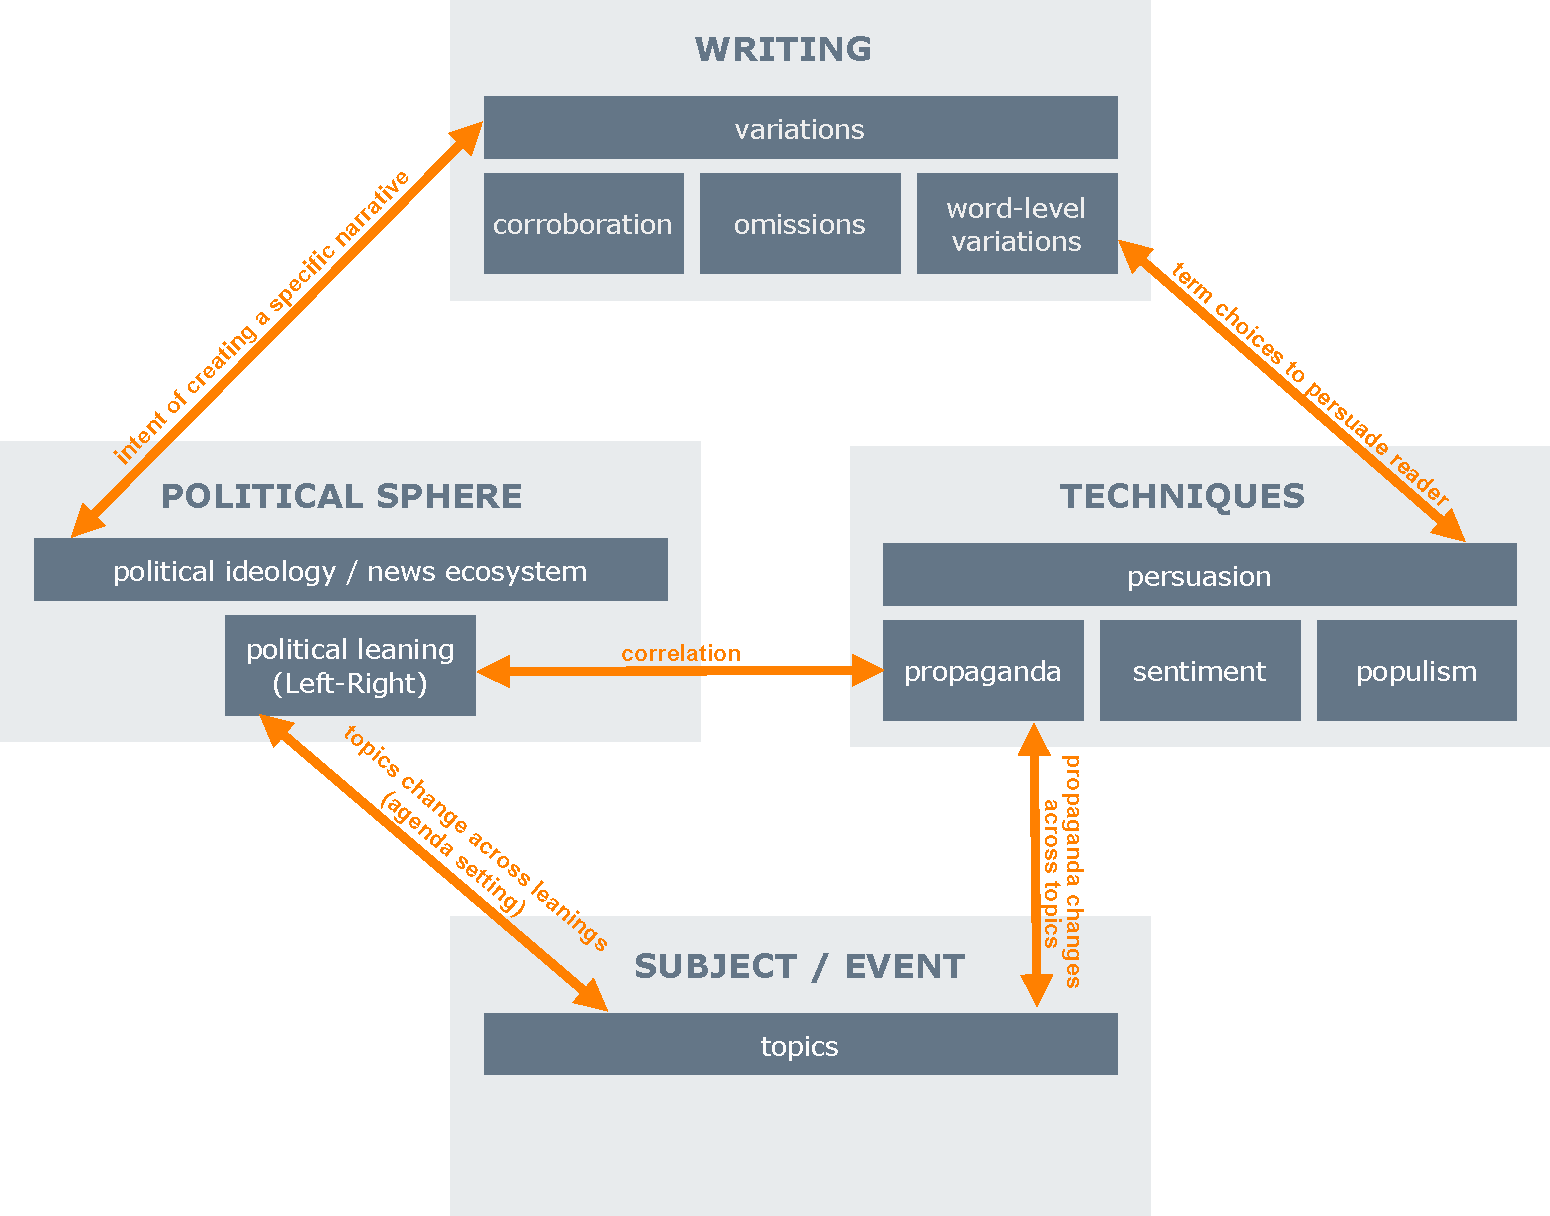
\includegraphics[width=\linewidth]{relationships.pdf}
    \caption{Relationships observed in this work}
    \label{fig:relationships}
\end{figure}

\begin{itemize}
    \item \emph{Word-level variations vs persuasion}: we have observed how different news outlets describe the same news event, by using words that are specifically selected to explicitly or implicitly elicit the reader’s emotional reaction. By observing triples of articles (AllSides dataset), we have seen how different terms are being used to provide multiple versions of the same story. These choices of terms, in many cases result in a variation of the detected techniques: both as resulting techniques, and as term importance.

    \item \emph{propaganda vs political leaning}: We observed this change of persuasive / propagandist language by taking into consideration the simplified categorisation by \emph{political leaning} (left/center/right) and tried to characterise linguistic profiles depending on this variable. Now, under the light of having redefined both the techniques and the political ideology, future works need to analyse how universal and specific linguistic patterns behave across different the different dimensions of political ideologies.

    \item \emph{political leaning vs topic}: We observed that the topics covered vary depending on the political leaning of the news sources. This is also a known effect from the literature, called \emph{agenda setting}~\citep{mccombs1972agenda}. By using the wider concept of political ideology, future works need to analyse how the topics change across the many dimensions of political ideologies.

    \item \emph{propaganda vs topic}: we observed that this variation of language is also very specific to the emph{topic}. Some topics are more controversial and find a higher quantity of propaganda, while others are more neutral and find less usage of linguistic techniques. Also here, as in the previous cases, we need to analyse how this relationship changes when we consider the wider concepts of linguistic patterns (universal vs specific) and political ideologies.
\end{itemize}

Our idea is that, in order to completely understand and model the relationships between these multiple variables, we need to use a \emph{multidimensional model} that can capture these relationships altogether. Modelling only relationships between couples of factors does not enable us to get a good understanding.

In Figure~\ref{fig:relationships} we have drawn different spheres, that relate to the experimental chapters of this Thesis. We started with this work to explore the connections between them, but as we can see, many of the relationships are still missing. These relationships need to be modelled in a joint effort from two different communities:

\begin{itemize}
    \item \emph{Social Sciences}: to understand the relationships between the political ideology of the news sources and the topics that they cover, and how this relates to the linguistic patterns that they use. This theoretical knowledge should drive the practical experimentation and help interpreting the results.
    \item \emph{Data Sciences}: to create a computational model and improve the techniques for tackling each one of the spheres.
\end{itemize}
The close collaboration and the exchange of knowledge between these two communities will be crucial to model the relationships between the considered dimensions.

% NEW RELATIONSHIPS:

% Once this is done, we can then try to focus more on the \emph{distinction} between persuasion and propaganda, at the intersection between social science (more conceptually) and data science.



\section{\statusgreen Final Remarks}
\label{sec:discussion_conclusions}

In this dissertation, we presented propaganda in relationships with multiple dimensions, such as political leaning, similarities across documents, and topics. Our analysis of these relationships was approached from multiple perspectives, which posed significant challenges. Nonetheless, these challenges served to make this doctoral work particularly engaging and rewarding.

From our contribution, we hope that the communities of researchers working on several computational news analysis tasks (e.g., propaganda detection, parallel news reports analysis and political leaning classification) can join their efforts and proceed in a research direction that would exploit the relationships that we described here in this work.
